\documentclass[a4paper]{article}

\usepackage[utf8]{inputenc}
\usepackage[francais]{babel}
\usepackage{hyperref}
\usepackage{graphicx}
\usepackage{fontspec} %Les accents disparaissent sans, je sais pas pourquoi...
\usepackage[textwidth=14cm]{geometry}
%\usepackage[textwidth=17cm,textheight=27cm]{geometry}

%\setlength{\textwidth}{420 pt} 
%\usepackage{amsmath}
%\usepackage{listings}
%\usepackage{moreverb}
%\usepackage{color}
%\usepackage[colorinlistoftodos]{todonotes}
%\usepackage[labelformat=empty]{caption}

\title{Systèmes multi-agents : la bille, le poisson et l'avatar}

\author{Matthieu CARON - Alexandre MOEVI}

\date{\today}

\begin{document}
\maketitle

\section{Architecture et utilisation}

\subsection{Usage}

En ouvrant l'archive, on peut constater dans le la présence de 4 répertoires : un \texttt{core} qui contient la base d'un système multi-agents et un pour chaque simulation (\texttt{particules}, \texttt{wator} et \texttt{game}). Chacun des trois simulations contient une classe Main pour lancer le programme.

Pour réaliser les différents simulations, il a été décidé d'utiliser la langage Python 3 et la bibliothèque graphique \href{https://wiki.python.org/moin/TkInter}{\texttt{Tkinter}}. On peut vérifier l'installation de Tkinter en lançant la commande \texttt{python3 -m tkinter} (ou \texttt{python -m tkinter}) ou l'installer avec \texttt{sudo apt-get install python3-tk} (ou chercher le nom du paquet avec \texttt{sudo apt-cache search tk}).

\medskip
La modification de la variable \texttt{\$PYTHONPATH} se fait directement dans chaque Main. Néanmoins si ça ne marche pas il faut faire les étapes suivantes.
Afin de permettre une architecture sous forme de paquetage en Python, il faut modifier la variable d'environnement \texttt{\$PYTHONPATH} en ajoutant le chemin vers le répertoire \texttt{sci} 

\medskip
\texttt{export PYTHONPATH=\$PYTHONPATH:/home/pmatthieu/example/tps/sci-caron-moevi}

\medskip
Sans cette modification, les imports ne marcheront pas. Cette modification peut être faite dans un terminal (méthode temporaire) ou directement dans les fichiers \texttt{.bashrc} et/ou \texttt{.bash\_profile}.

\medskip
modifier les paramètres dans MainXXX.py, etc.

\subsection{Paquetage \texttt{core}}
Avant d'expliquer les trois simulations effectuées, il est nécessaire de présenter le paquetage \texttt{core}. \texttt{core} contient la description générique des objets nécessaires à la mise d'un SMA (système multi-agents). Le paquetage contient cinq classes.
 
\medskip
La classe \texttt{Agent} qui représente un agent du système. Placé dans un \texttt{Environnement}, il connaît ses coordonnées (\texttt{self.x} et \texttt{self.x} en Python, qui correspondent à \texttt{this.x} et \texttt{this.y} en Java). Quand le \texttt{SMA} lui \og donne la parole \fg{}, l'agent décide en fonction de stratégie (méthode \texttt{self.decide()}) puis se met à jour dans son environnement (\texttt{self.update()}). L'agent possède également une méthode \texttt{place\_agent()} qui concerne son affichage dans la fenêtre (classe \texttt{Window}).

\medskip
La classe \texttt{AgentCreator} génère un ou plusieurs \texttt{Agent} du système. Il peut créer un seul type d'agent (uniquement des billes) ou plusieurs types d'agents (poissons et requins).

\medskip
La classe \texttt{Environnement} représente l'espace du système sous forme de grille. Cette grille contient l'ensemble des agents et leur coordonnées. L'environnement peut être torique ou non. 

\medskip
La classe \texttt{SMA} est la classe qui controle tout, à l'initialisation elle va créer un environnement et va faire nbAgents appels à la méthode create de la classe AgentCreator.
La classe \texttt{SMA} contient la méthode \texttt{run()} qui effectue le tour de parole (ou tick). Dans un tick, le \texttt{SMA} appelle un ou plusieurs agents avec la méthode \texttt{agent.decide()} en fonction du scheduling (\texttt{self.scheduling}). Le scheduling peut être séquentiel, équitable ou aléatoire. Un fois le tour fini, l'affichage est mis à jour avec la méthode \texttt{SMA.updateDisplay()}.

\medskip
La classe \texttt{Window} concerne tout ce qui l'affichage. En se basant sur la bibliothèque graphique \texttt{Tkinter}, la classe permet l'affichage du système et l'affichage d'une grille si l'utilisateur le souhaite.

\section{Simulations}

\subsection{Tube à particules}

La première simulation, le paquetage \texttt{particules}, reproduit le comportement de billes (ou particules) dans un espace. Cet espace peut torique ou non ; s'il ne l'est pas, les particules rebondissent contre les murs. Les particules rebondissent également en collision.

\medskip
La classe \texttt{Bille} hérite la classe \texttt{Agent} du paquetage \texttt{core}. L'agent \texttt{Bille} connaît son environnement, sa position (entiers \texttt{x} et \texttt{y}) et sa direction (vecteur à 2 dimensions \texttt{[a, b]}).

\medskip
La stratégie d'une particule est la suivante :
\begin{itemize}
\item Dans la méthode \texttt{nextPos()}, la particule calcule sa prochaine possible destination en fonction de l'espace torique (apparition de \og l'autre côté \fg{} de l'écran) ou non (rebond).
\item Dans \texttt{decide()}, la particule regarde sa prochaine destination. Si la voie est libre, elle se prépare à se déplacer (\texttt{particule.bougera = True}). Sinon ça veut dire qu'elle essaye de se rendre dans une case occupée par une autre particule : c'est une collision.
\item Dans \texttt{update()}, si la particule peut bouger, elle se met à sa nouvelle position en laissant libre son ancienne place et l'environnement se met à jour.
\end{itemize}

\medskip
Dans le cas d'une collision (\texttt{particule1.collision(particule2)}), la bille \og incidente \fg{}, c'est-à-dire celle qui essaye d'aller dans une case déjà occupée, échange sa direction avec l'autre particule. Il a été décidé que la bille incidente ne se déplace pas pendant le tick de collision, malgré sa nouvelle direction. Afin d'avoir un comportement cohérent lorsque les billes remplissent la grille et donc qu'elles ne peuvent pas bouger.
 
\begin{figure}[!h]
\centering
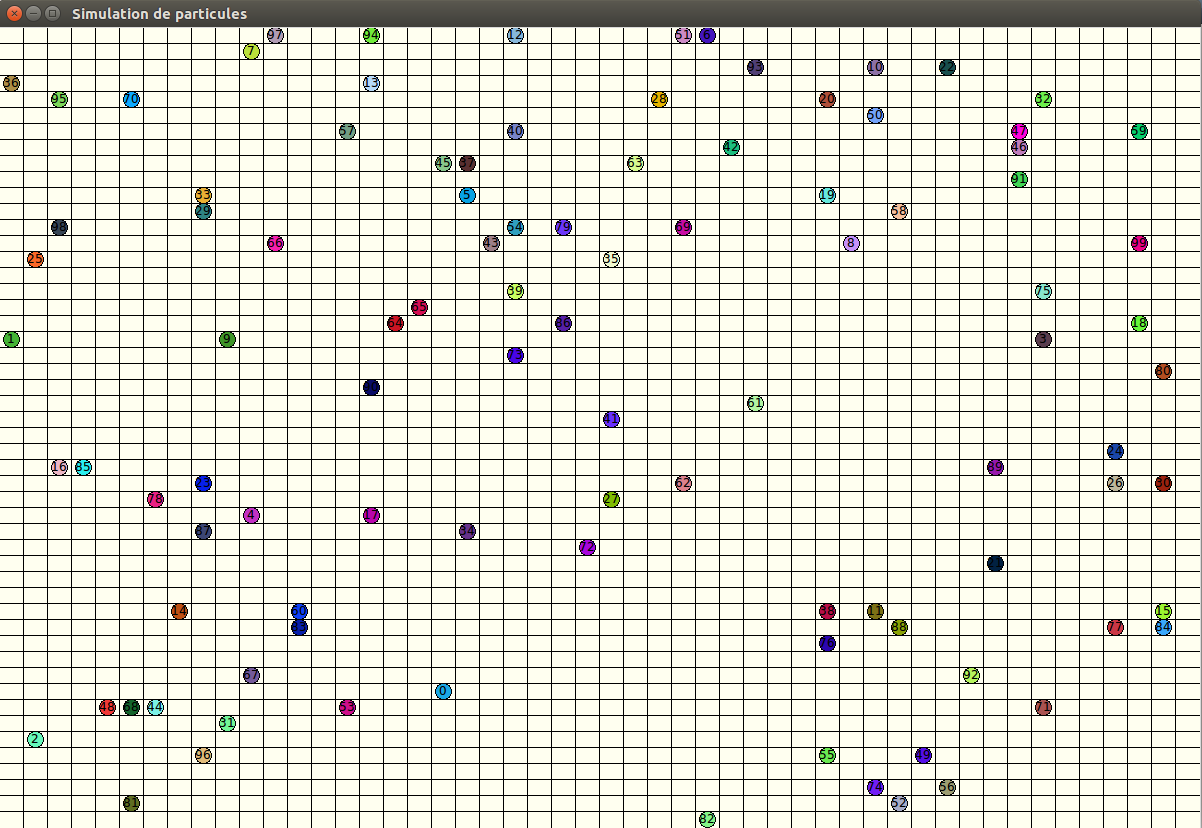
\includegraphics[height=7cm]{particules.png}
\caption{Fenêtre d'exécution du programme \texttt{MainBille}. Les billes sont assignées d'une couleur aléatoire et d'un identifiant pour faciliter leur suivi.}
\end{figure}

\subsection{Poissons et requins dans le golfe (du Bénin)}
La deuxième simulation concerne le paquetage \texttt{wator}. Elle a pour but de voir comment des poissons (les agents \texttt{Fish} dans notre simulation) et des requins (agents \texttt{Shark}) cohabitent dans une zone. 

\medskip
Un agent \texttt{Fish} se déplace de façon aléatoire et se reproduit tous les \texttt{fishBreedTime} ticks. Pour se reproduire, le poisson doit se déplacer et donne naissance à un autre poisson sur la case où il était précédemment. Il observe donc dans le voisinage de Moore les cases qui sont libres et en prend une au hasard si c'est possible. Enfin l'âge augmente de 1 à chaque tick.

\medskip
Un \texttt{Shark} est affamé, il a \texttt{dontStarve} ticks pour manger un \texttt{Fish}. S'il n'y arrive pas à temps, il meurt. À l'instar du poisson, il peut se reproduire tous les \texttt{sharkBreedTime} et donne naissance à un nouveau requin sur la case qu'il occupait avant.

\medskip
Comme pour l'agent \texttt{Bille} de la simulation précédente, les agents \texttt{Fish} et \texttt{Shark} ont conscience de leur environnement et connaissent leur coordonnées dans l'espace.

\medskip
Avec ces paramètres, le but est de trouver d'atteindre une situation d'équilibre. On veut éviter une pénurie de poissons (plus de poissons = mort des requins affamés = zone vierge de tout animal) et une absence de requins (les poissons vont se reproduire jusqu'à remplir entièrement la zone).

\medskip
La classe \texttt{FishAndSharkCreator} prend en paramètres un nombre de \texttt{Shark} et un nombre de \texttt{Fish}. Chaque appel à la méthode \texttt{FishAndSharkCreator.create(x,y)} renvoie aléatoirement un \texttt{Fish} ou un \texttt{Shark} qui sera placé aux coordonnées \texttt{x} et \texttt{y} dans un \texttt{Environnement}. Les coordonnées données en paramètre sont générées de façon aléatoire et renvoient vers une case vide qui sera occupé par le nouvel agent.
 
\begin{figure}[!h]
\centering
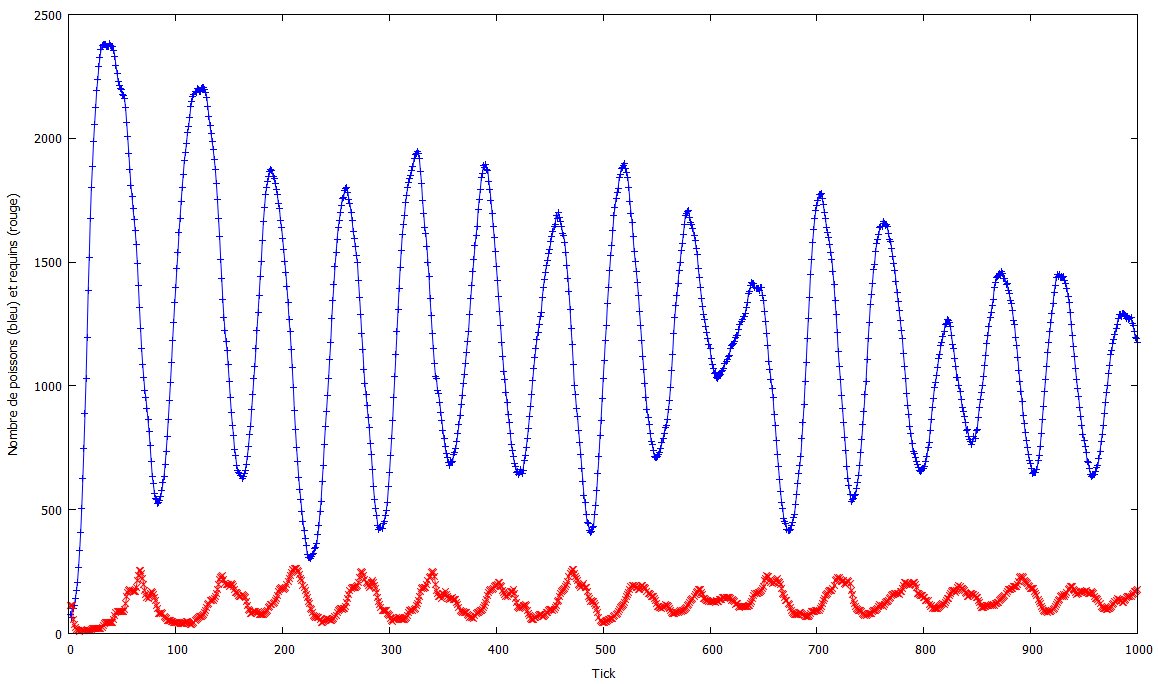
\includegraphics[height=7cm]{1000tours.png}
\caption{Courbes de population.}
\end{figure}

\subsection{Pâques-Manne, ou l'histoire de chasseurs chassant un avatar}
Enfin dans cette simulation correspondant au paquetage \texttt{game}, le système s'inspire du jeu vidéo des années 1980 \textit{Pac-Man}. 

\medskip
L'utilisateur contrôle au clavier un agent \texttt{Avatar}. Le but en tant qu'\texttt{Avatar} est de ne pas se faire attraper par les \texttt{Hunters} sinon la partie est perdue. Pour gagner, le joueur peut dévorer tous les \texttt{Hunters} ou prendre le \texttt{Winner} qui apparaît une fois que l'\texttt{Avatar} ait mangé suffisamment de \texttt{Defender}. En mangeant un \texttt{Defender}, le joueur est invincible pendant un certain temps et peut dévorer les \texttt{Hunters} qui tentent de fuir.

\medskip
Un agent \texttt{Avatar} se déplace en fonction du dernier input (gauche, droite, haut ou bas) du joueur. Si l'\texttt{Avatar} fonce dans un mur il ne se déplace plus et attend que le joueur donne une nouvelle direction. Enfin à chaque prise de parole, l'agent va calculer sa matrice de Dijkstra (\texttt{Avatar.update()}) qui sera enregistrée dans l'\texttt{Environnement} ; tous les \texttt{Hunter} peuvent ainsi y accéder et voir quel case les rapprochent de l'\texttt{Avatar}.

\medskip
Un agent \texttt{Hunter} se déplace en fonction de la matrice de Dijkstra et des autres agents (il n'ira pas dans un mur ni dans un autre \texttt{Hunter} mais ira tuer l'\texttt{Avatar}) en choisissant uniquement une position améliorante (avec un score strictement inférieur à sa position actuelle, l'inverse si l'\texttt{Avatar} est invulnérable). Parmi les futures positions améliorantes avec le même score, il en choisit une de libre au hasard pour éviter de privilégier tous les déplacements vers une direction (par exemple, l'agent pourrait d'abord regarder toujours vers le bas).

\medskip
Un agent \texttt{Defender} apparait à un emplacement aléatoire vide sur la map et reste en vie \texttt{defenderLife} tours. Il permet de donner une invincibilité temporaire à l'\texttt{Avatar} et a pour conséquence de changer la stratégie des \texttt{Hunter} (\texttt{Hunter.doitFuir = True}).

\medskip
Enfin, un agent \texttt{Wall} qui est placé à la création de l'environnement et influe sur le calcul de la matrice de Dijkstra. \texttt{nbWalls} murs sont placés de manière aléatoire dans l'\texttt{Environnement}.

\subsubsection{Remarques sur le GameAgentCreator}
Le SMA à l'initialisation appelle \texttt{nbAgents} fois la méthode \texttt{create} de la classe \texttt{GameAgentCreator} et ajoute ces agents à l'environnement avec la méthode \texttt{ajouteAgent(Agent)} de la classe \texttt{Environnement}. Il y a deux remarques que l'on pourrait faire.

\medskip
Le premier est l'intérêt de donner la parole aux agents \texttt{Wall}. Une fois placé à la création, le mur est un élément qui ne décide de rien (\texttt{decide()}) et qui n'a pas besoin de se mettre à jour (\texttt{update()}). Même si le jeu est fluide sur les différents tests effectués, ne pas donner la parole aux murs permettrait un gain de performance.

\medskip
Le deuxième problème est la génération des agents. \texttt{GameAgentCreator} recherche une place libre aléatoire et peut placer des agents \og entre quatre murs \fg{}. Dans le meilleur des cas, l'\texttt{Avatar} peut quand même atteindre les \texttt{Defender} et prendre le Winner pour finir le jeu.  Dans le pire de cas, l'\texttt{Avatar} est isolé et, puisqu'il n'y a pas de chemin possible entre les chasseurs et le joueur ET que le \texttt{Winner} est apparu en dehors de la zone accesible par l'\texttt{Avatar}, le joueur ne peut ni perdre ni gagner. Discutée pendant le développement, la génération procédurale de labyrinthe de n'a pas été implémentée.

\end{document}